\documentclass{article}
\usepackage{tikz}
\usetikzlibrary{arrows.meta, backgrounds}

\begin{document}

\begin{figure}[h]
    \centering
    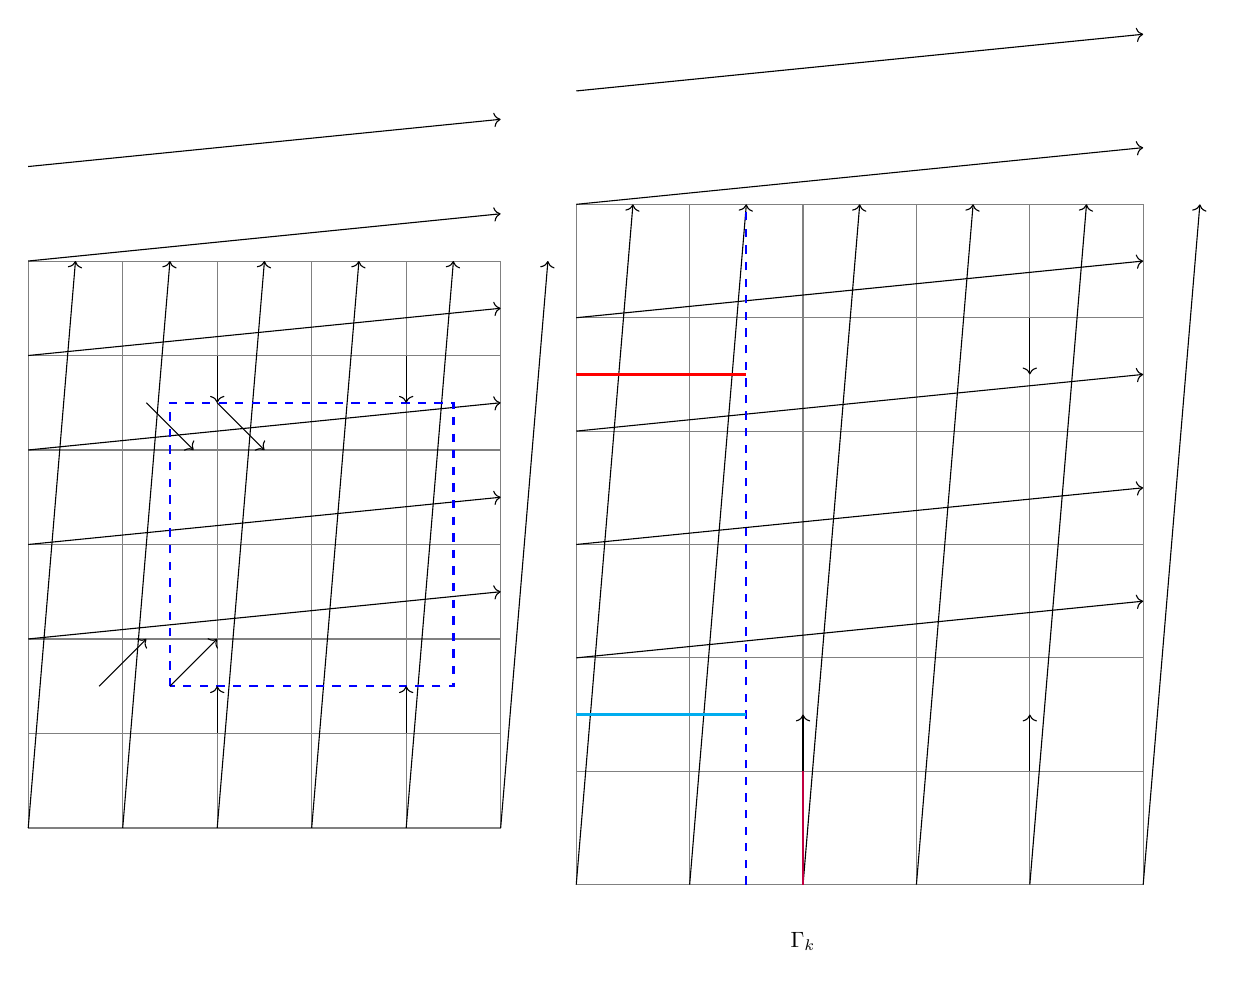
\begin{tikzpicture}[scale=1.2, every node/.style={scale=0.8}]

        % Left Diagram
        \draw[gray] (-1,-3) grid (4,3);
        \foreach \x in {-1,...,4}{
            \draw[->] (\x,-3) -- ({\x+0.5},3);
            \draw[->] (-1,\x) -- (4,{\x+0.5});
        }
        \draw [blue,dashed,thick]  (.5,-1.5) rectangle ++(3,3);  % blue region
        \foreach \x in {0.5,2}{
            \draw[black,->] (0.5*\x,-1.5) ++(-0.5,0) -- ++(0.5,0.5);
            \draw[black,->] (0.5*\x,1.5) -- ++(0.5,-0.5);
        }
        \foreach \x in {1,3}{
            \draw[black,->] (\x,-1.5) ++(0,-0.5) -- ++(0,0.5);
            \draw[black,->] (\x,1.5) ++(0,0.5) -- ++(0,-0.5);
        }

        % Right Diagram
        \begin{scope}[xshift=6cm,scale=1.2]
            \draw[gray] (-1,-3) grid (4,3);
            \foreach \x in {-1,...,4}{
                \draw[->] (\x,-3) -- ({\x+0.5},3);
                \draw[->] (-1,\x) -- (4,{\x+0.5});
            }
            \draw [blue,dashed,thick]  (0.5,-3) -- (0.5,3);  % blue region
            \draw [cyan,thick]  (-1,-1.5) -- (0.5,-1.5);
            \draw [red,thick]  (-1,1.5) -- (0.5,1.5);
            \draw [purple,thick]  (1,-3) -- (1,-1.5);
            \draw[black,->] (1,-1.5) ++(0,-0.5) -- ++(0,0.5);
            \draw[black,->] (3,-1.5) ++(0,-0.5) -- ++(0,0.5);
            \draw[black,->] (3,1.5) ++(0,0.5) -- ++(0,-0.5);
            \node at (1,-3.5) {$\Gamma_{k}$};
        \end{scope}

    \end{tikzpicture}
    \caption{Left: The setup for the Gibbs property in the uncolored $q$-Boson model. Outgoing arrow counts outside the region $\Lambda$ outlined in blue are conditioned upon, and arrows have been displayed in this depiction if the arrow count is non-zero and has been conditioned on. Arrow counts entering the blue region are conditioned on due to consistency, but those exiting it are not. Right: The setup for the Gibbs property in the colored $q$-Boson model. Horizontally outgoing colored arrows counts are conditioned on strictly to the left of the blue dashed line (which extends to the ends of the domain in both directions), while only total outgoing arrow counts (depicted in black) are conditioned on to the right (including on $\Gamma_k$).}
    \label{fig:gibbs_property}
\end{figure}

\end{document}